\begin{frame}{Nominal Price Graphs}
\begin{figure} [H]
	\begin{center}
		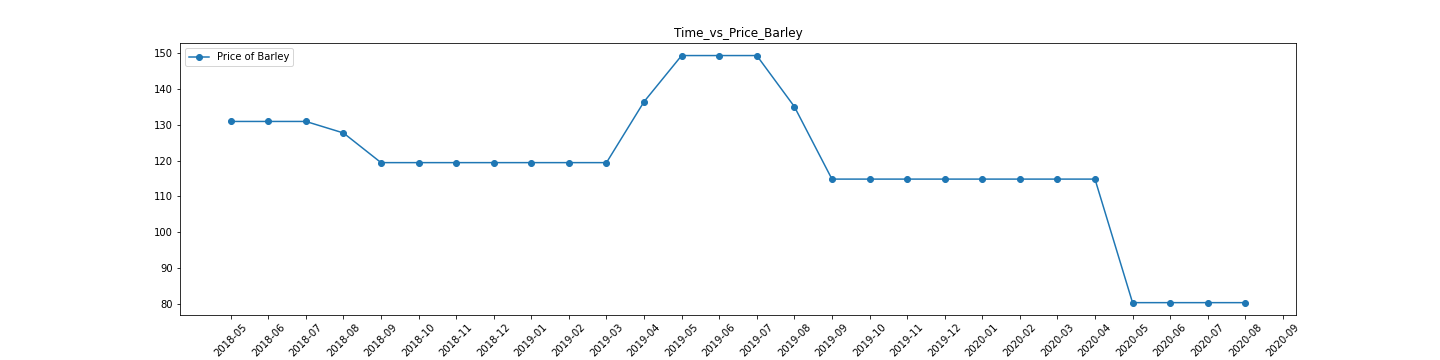
\includegraphics[scale=0.2]{images/illustrate/Time_vs_Price_Barley.png}
	\end{center}
	\caption{Price of barley in nominal values}
	\label{fig:log-archi}
\end{figure}
\begin{figure} [H]
	\begin{center}
		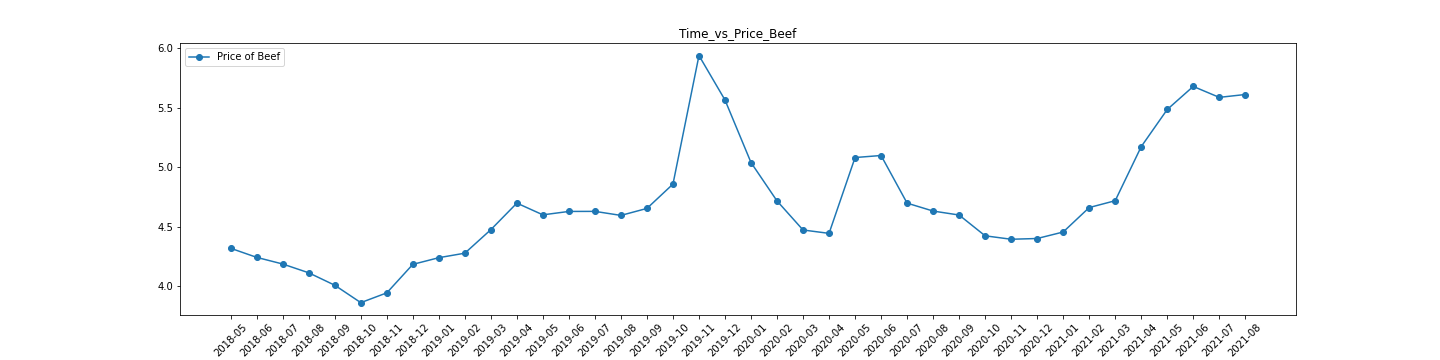
\includegraphics[scale=0.2]{images/illustrate/Time_vs_Price_Beef.png}
	\end{center}
	\caption{Price of beef in nominal values}
	\label{fig:log-archi}
\end{figure}
    
\end{frame}
\begin{frame}{Nominal Price Graphs}
    \begin{figure} [H]
	\begin{center}
		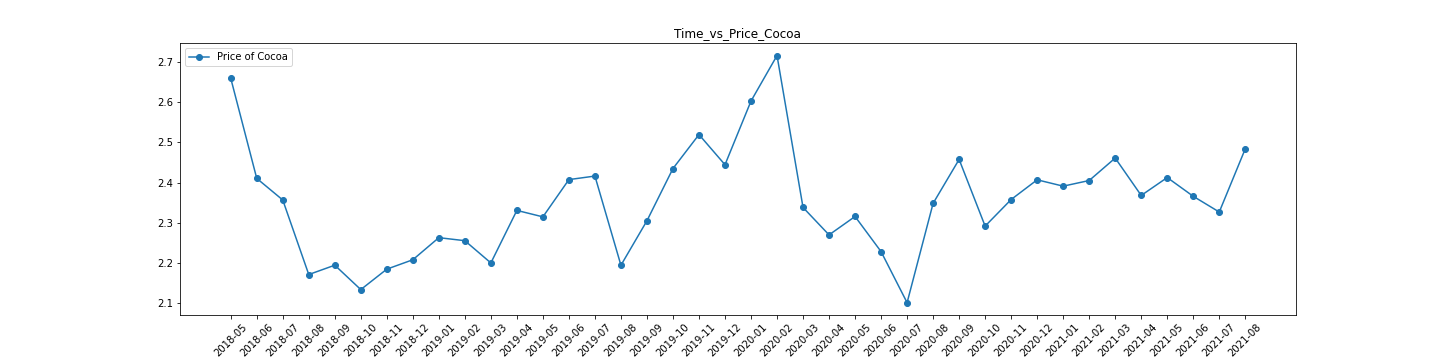
\includegraphics[scale=0.2]{images/illustrate/Time_vs_Price_Cocoa.png}
	\end{center}
	\caption{Price of cocoa in nominal values}
	\label{fig:log-archi}
\end{figure}
\begin{figure} [H]
	\begin{center}
		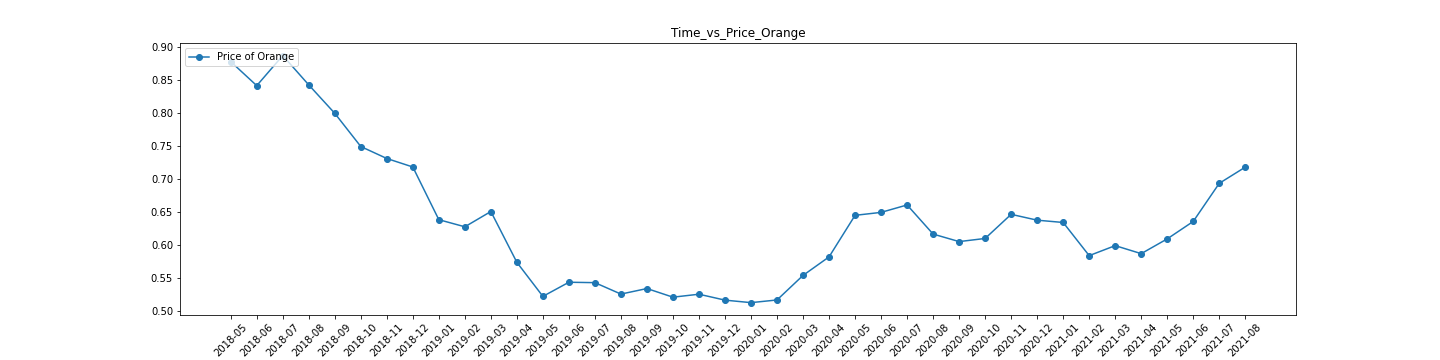
\includegraphics[scale=0.2]{images/illustrate/Time_vs_Price_Orange.png}
	\end{center}
	\caption{Price of orange in nominal values}
	\label{fig:log-archi}
\end{figure}
\end{frame}

\begin{frame}{Nominal Price Graphs}
  \begin{figure} [H]
	\begin{center}
		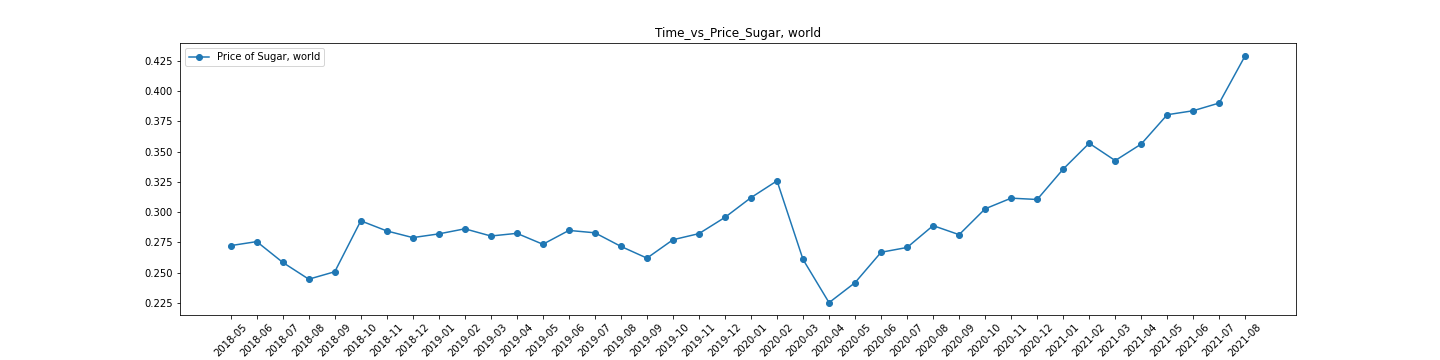
\includegraphics[scale=0.2]{images/illustrate/Time_vs_Price_Sugar, world.png}
	\end{center}
	\caption{Price of sugar in nominal values}
	\label{fig:log-archi}
\end{figure}
\begin{figure} [H]
	\begin{center}
		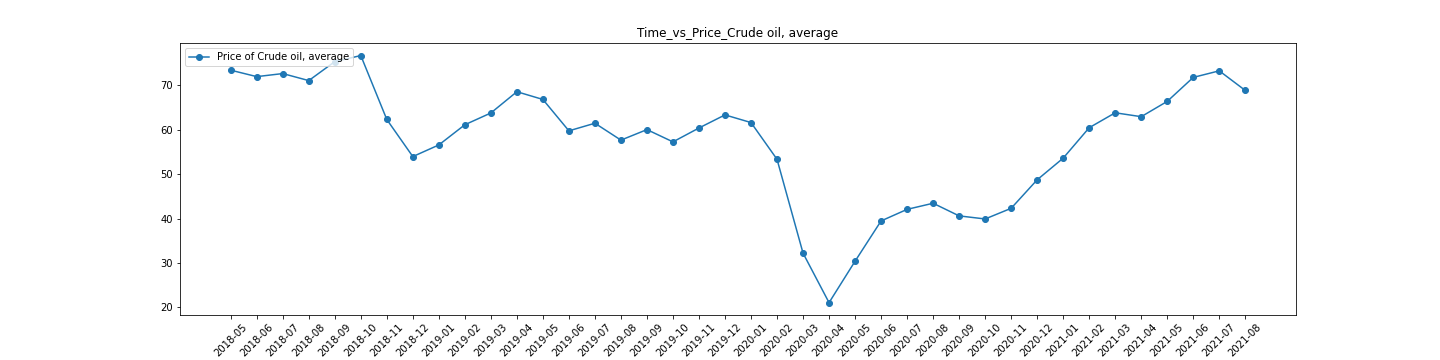
\includegraphics[scale=0.2]{images/illustrate/Time_vs_Price_Crude oil, average.png}
	\end{center}
	\caption{Price of crude oil in nominal values}
	\label{fig:log-archi}
\end{figure}
\end{frame}

\begin{frame}{Nominal Price Graphs}
  \begin{figure} [H]
	\begin{center}
		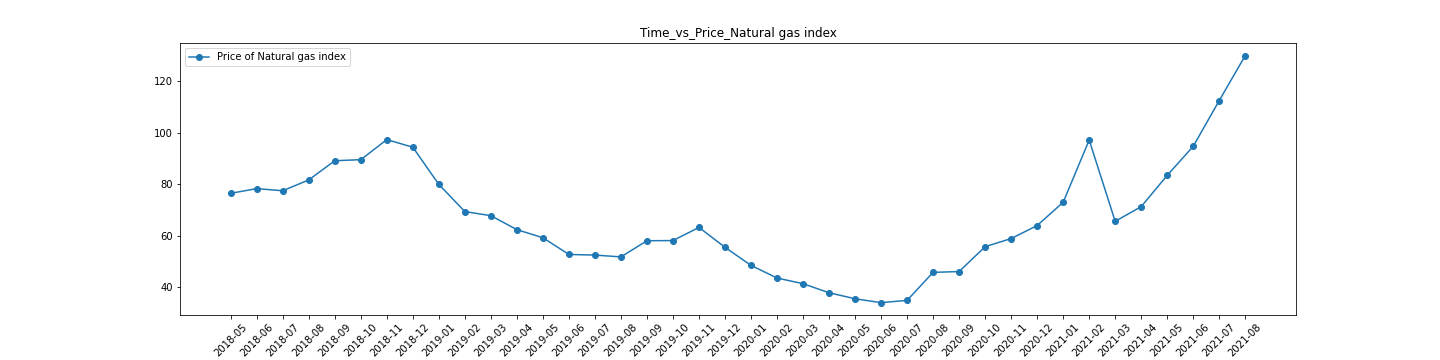
\includegraphics[scale=0.2]{images/illustrate/Time_vs_Price_Natural gas index.png}
	\end{center}
	\caption{Price of natural gas in nominal values}
	\label{fig:log-archi}
\end{figure}
\begin{figure} [H]
	\begin{center}
		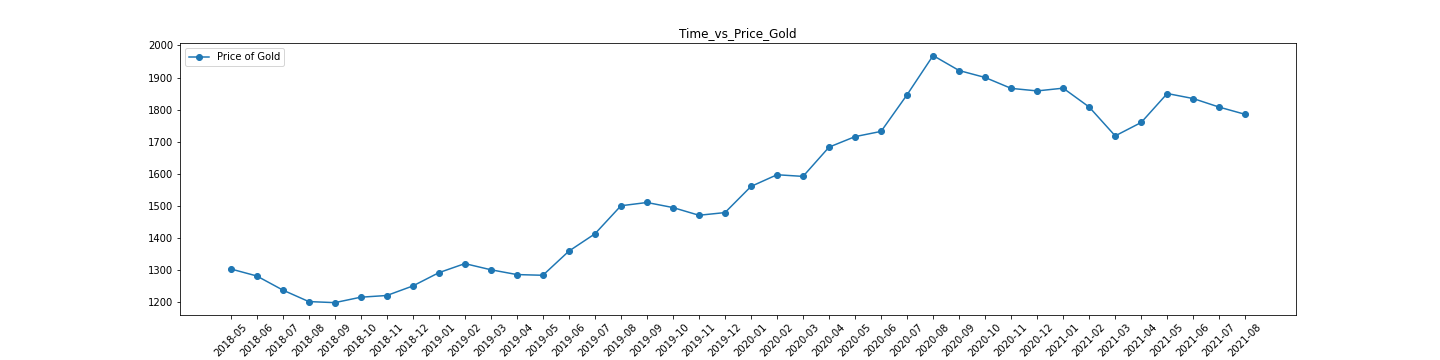
\includegraphics[scale=0.2]{images/illustrate/Time_vs_Price_Gold.png}
	\end{center}
	\caption{Price of gold in nominal values}
	\label{fig:log-archi}
\end{figure}
\end{frame}


\begin{frame}{Figure for G20 inflation with respect to time}
  \begin{figure} [H]
	\begin{center}
		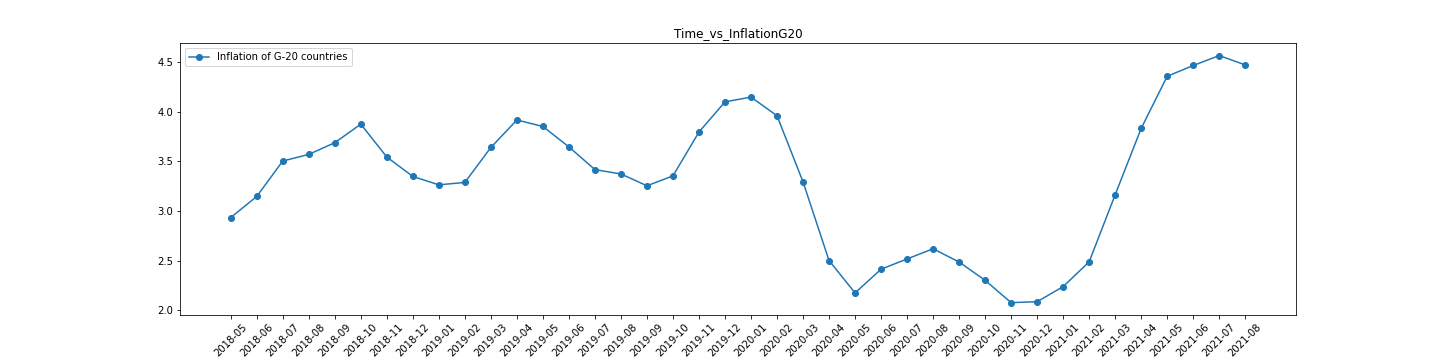
\includegraphics[scale=0.2]{images/illustrate/Time_vs_InflationG20.png}
	\end{center}
	\caption{G20 inflation with respect to time}
	\label{fig:log-archi}
\end{figure}

\end{frame}

\begin{frame}{Percentage Change Graphs}
 \begin{figure} [H]
	\begin{center}
		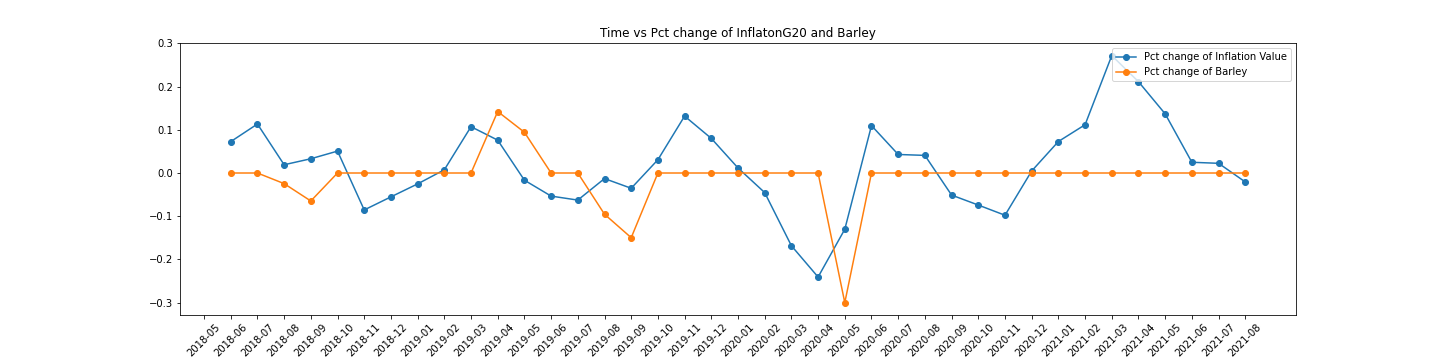
\includegraphics[scale=0.2]{images/illustrate/pct_change_inflation_and_Barley.png}
	\end{center}
	\caption{Percentage change of barley in comparison to G20 inflation }
	\label{fig:log-archi}
\end{figure}

\begin{figure} [H]
	\begin{center}
		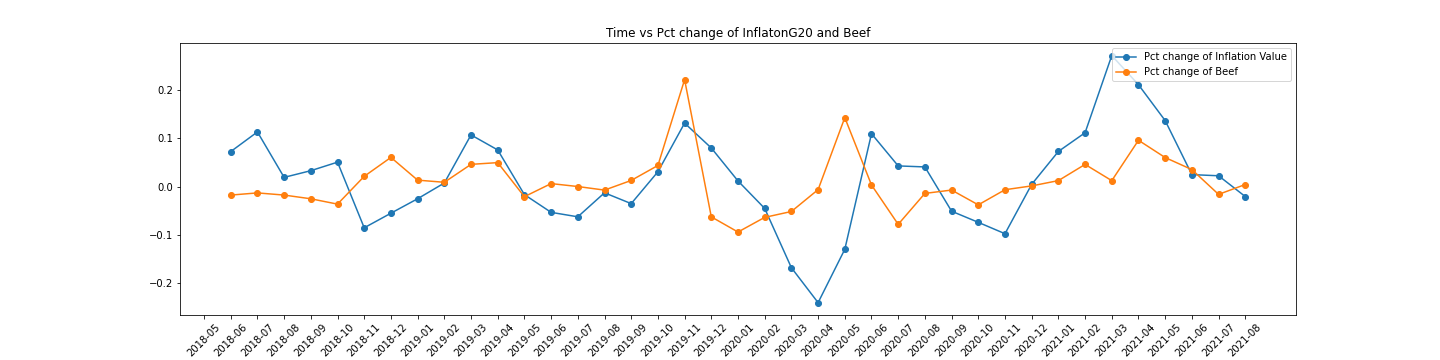
\includegraphics[scale=0.2]{images/illustrate/pct_change_inflation_and_Beef.png}
	\end{center}
	\caption{Percentage change of beef in comparison to G20 inflation  }
	\label{fig:log-archi}
\end{figure}
\end{frame}


\begin{frame}{Percentage Change Graphs}
    \begin{figure} [H]
	\begin{center}
		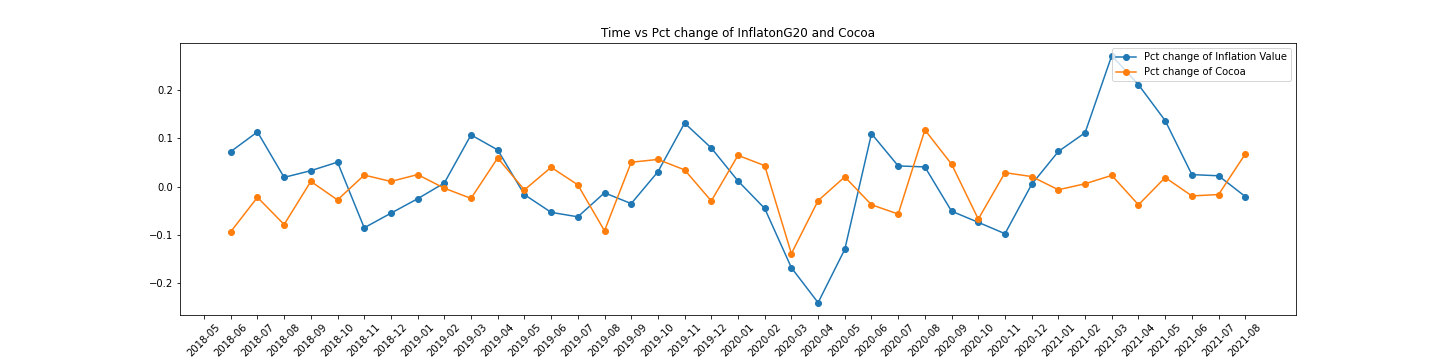
\includegraphics[scale=0.2]{images/illustrate/pct_change_inflation_and_Cocoa.png}
	\end{center}
	\caption{Percentage change of cocoa in comparison to G20 inflation  }
	\label{fig:log-archi}
\end{figure}


\begin{figure} [H]
	\begin{center}
		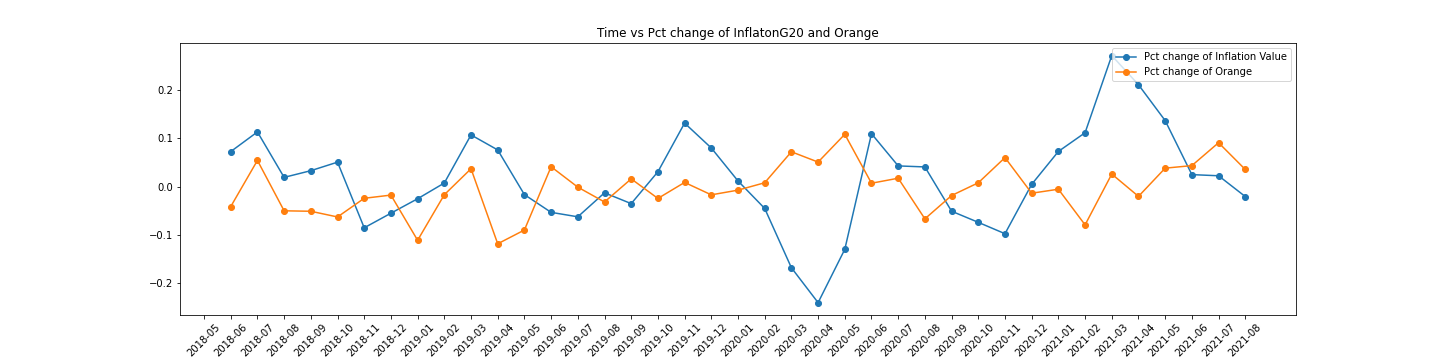
\includegraphics[scale=0.2]{images/illustrate/pct_change_inflation_and_Orange.png}
	\end{center}
	\caption{Percentage change of orange in comparison to G20 inflation  }
	\label{fig:log-archi}
\end{figure}

\end{frame}



\begin{frame}{Percentage Change Graphs}
 \begin{figure} [H]
	\begin{center}
		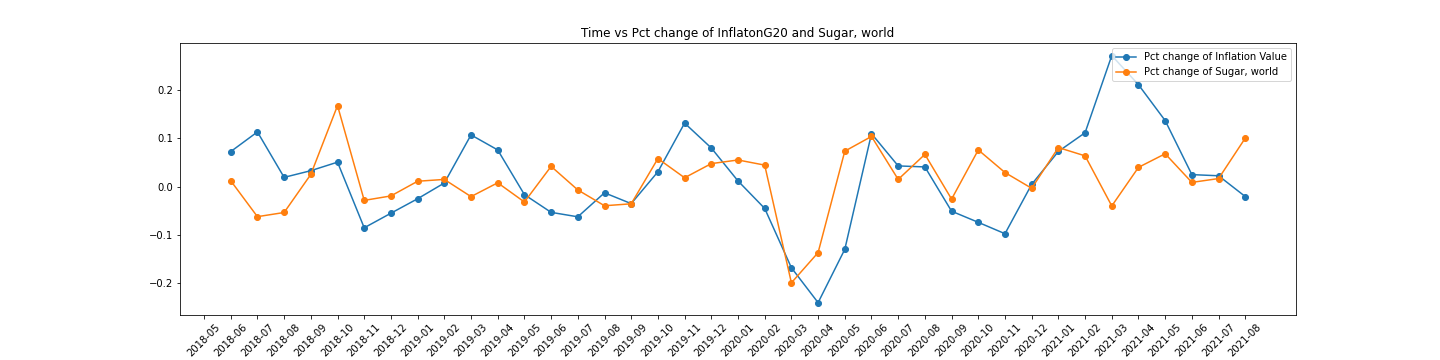
\includegraphics[scale=0.2]{images/illustrate/pct_change_inflation_and_Sugar, world.png}
	\end{center}
	\caption{Percentage change of sugar in comparison to G20 inflation  }
	\label{fig:log-archi}
\end{figure}


\begin{figure} [H]
	\begin{center}
		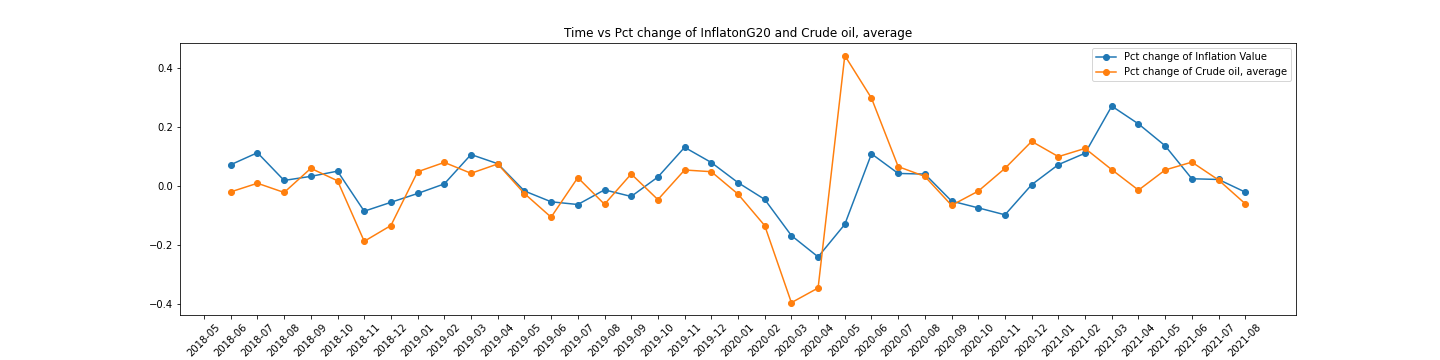
\includegraphics[scale=0.2]{images/illustrate/pct_change_inflation_and_Crude oil, average.png}
	\end{center}
	\caption{Percentage change of crude oil in comparison to G20 inflation  }
	\label{fig:log-archi}
\end{figure}

\end{frame}

\begin{frame}{Percentage Change Graphs}
 \begin{figure} [H]
	\begin{center}
		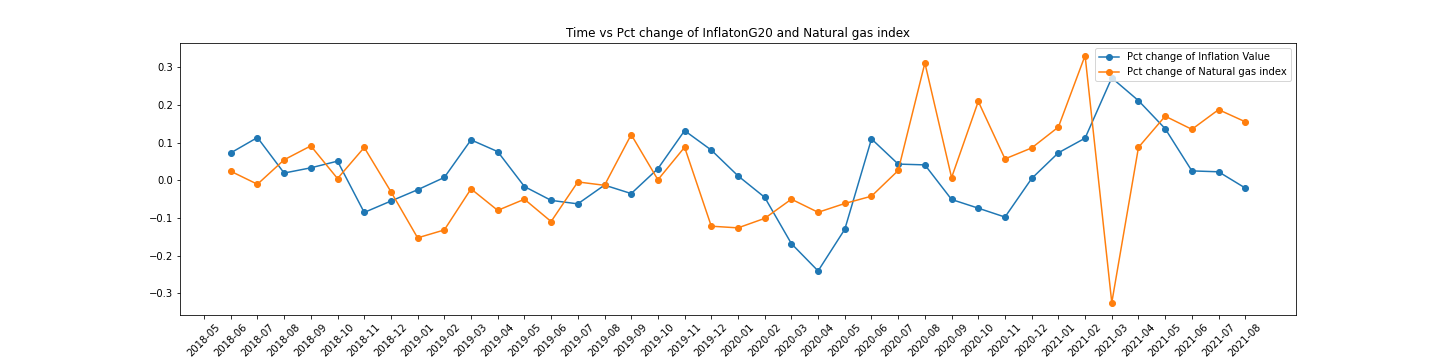
\includegraphics[scale=0.2]{images/illustrate/pct_change_inflation_and_Natural gas index.png}
	\end{center}
	\caption{Percentage change of natural gas in comparison to G20 inflation  }
	\label{fig:log-archi}
\end{figure}

\begin{figure} [H]
	\begin{center}
		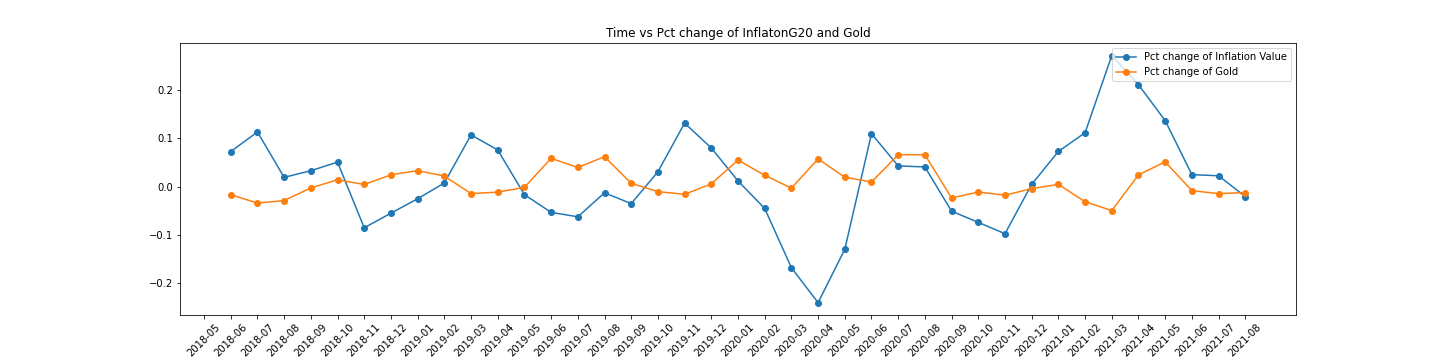
\includegraphics[scale=0.2]{images/illustrate/pct_change_inflation_and_Gold.png}
	\end{center}
	\caption{Percentage change of gold in comparison to G20 inflation  }
	\label{fig:log-archi}
\end{figure}

\end{frame}

\begin{frame}{Percentage Change of All Commodities vs Inflation}
    \begin{figure} [H]
	\begin{center}
		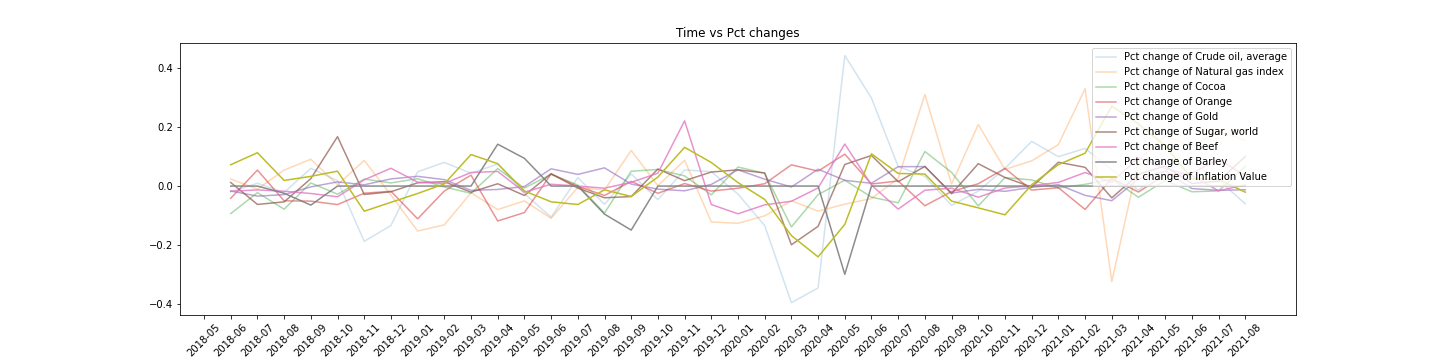
\includegraphics[scale=0.2]{images/illustrate/pct_changes_together.png}
	\end{center}
	\caption{Percentage change of all commodities in comparison to G20 inflation  }
	\label{fig:log-archi}
\end{figure}
\end{frame}


\begin{frame}{Result}

        \begin{enumerate}
            \item From the previous graphs we can see that not all commodity prices increase faster than inflation rate. Clearly there is a strong positive correlation between most of the commodity prices and inflation.
            \item  However, from figure percentage change of all commodities, we can see that not all commodity prices increase faster than inflation. 
            \item To conclude, our analysis display that general trend of inflation and commodity prices are posi- tively correlated. However, there is no clear evidence which supports the statement commodity prices grow faster than global inflation.
            
        \end{enumerate}

  
\end{frame}

\begin{frame}{Result}

        \begin{enumerate}
           
            \item At some time intervals, commodities dominate the rate of increase in inflation value and vice versa.
            \item In other words, since we have not observed any consistent pattern, the question "Do commodity prices grow faster than global inflation?" can not be answered directly and depends on the small monthly intervals.
        \end{enumerate}

  
\end{frame}